\documentclass[11pt, a4paper]{article}

\usepackage{graphicx}
\usepackage[a4paper,top=3cm,bottom=2cm,left=2cm,right=2cm,marginparwidth=1.75cm]{geometry}
\usepackage[english]{babel}
\usepackage[utf8x]{inputenc}
\usepackage{subfig}
\usepackage{float}
\usepackage{amsmath}
\usepackage{amssymb}
\usepackage{mhchem}
\usepackage{hyperref}
\usepackage{tikz}
\usepackage{cancel}

\graphicspath{ {./images} }
\newcommand*{\qed}{\hfill\ensuremath{\quad\square}}%
\newcommand*{\rad}{\ensuremath{\,\text{rad}}}
\newcommand*{\R}{\ensuremath{\mathbb{R}}}
\newcommand*{\C}{\ensuremath{\mathbb{C}}}
\renewcommand*{\Re}{\operatorname{Re}}
\renewcommand*{\Im}{\operatorname{Im}}
\renewcommand*{\epsilon}{\varepsilon}
\renewcommand*{\phi}{\varphi}

\makeatletter
\renewcommand*\env@matrix[1][*\c@MaxMatrixCols c]{%
  \hskip -\arraycolsep
  \let\@ifnextchar\new@ifnextchar
  \array{#1}}
\makeatother

\newtheorem{theorem}{Theorem}

%------------------------------------------------
%Templates for images and figures
% \begin{figure}[h]
%   \centering
%   \subfloat[caption 1]{{
\includegraphics[width=30mm]{images/placeholder.png}}}%
%   \qquad
%   \subfloat[caption 2]{{
\includegraphics[width=30mm]{images/placeholder.png}}}%
%   \caption{Description}
% \end{figure}

% \begin{figure}[h]
%   \centerline{
\includegraphics[width=50mm]{images/placeholder.png}}
%   \caption{Description}
% \end{figure}

%Template for a simple table 
%\begin{table}[h]
%   \caption{Description} %title of the table
%   \centering % centering table
%   \begin{tabular}{l rr} % creating three columns
%     \hline\hline %inserting double-line
%     & & \\ [0.5ex] % Insert half line vertical spacing
%     \hline % inserts single-line
%     & & \\ 
%     & & \\
%     & & \\
%     & & \\
%   \hline % inserts single-line
%   \end{tabular}
%   \label{tab:hresult}
% \end{table}
%-----------------------------------------------

\begin{document}
\setcounter{section}{4}
\setcounter{equation}{0}

\section{WOP3B Lecture 5: Influencing material proerties through manufacturing}

\subsection{Introduction}
Fabrication of materials into work affects the microstructure. We've seen before that microstructure largely dictates mechanical properties. Thus material properties are influenced by the manufacturing processes used. This applies to all materials though it's most important for metals and ceramics to a lesser extent. Fabrication processes of metals can be divided into $3$ main groups: forming operations such as forging and drawing, casting and miscellaneous operations such as welding and powder mettalurgy.


\subsection{Casting of metals}
When casting liquid metal is added to some kind of mold. It solidifies within the mold. When the mold is removed the casting is left. There are many different types of casting such as injection molding, sand casting, die casting and lost-wax casting.\\
\\
Metals will start to solidify when the Gibbs free energy ($G$) of the solid is lower then that of the liquid. For pure metals this happens when $T = T_m$ where $T_m$ is the melting point. When cooling happens very quickly the driving force for solidification increases. This causes greater amounts of crystalization inside the fluid. This in turn leads to a finer grain structure when completely solidified.\\
\\
Metals usually have a high thermal conductivity. Thus when casting in a metal mold cooling happens faster since the mold transfers heat away from the work faster. As asserted before this results in finer grains when compared to for example a sand mold. Recall from the lecture on welding that grains tend to grow in the direction of the highest thermal gradient. In case of a metal mold this is from inside the work to the surface of the work as the surface is in contact with the metal mold. Because of this the core of the work has larger grains.
\begin{figure}[h]
  \centering
  \subfloat[Metal mold]{{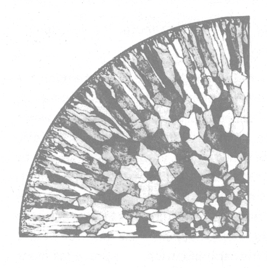
\includegraphics[width=50mm]{images/MetalMold.png}}}%
  \qquad
  \subfloat[Sand mold]{{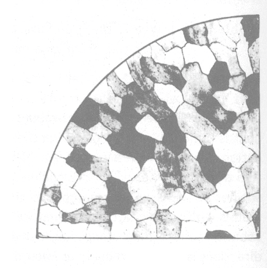
\includegraphics[width=50mm]{images/SandMold.png}}}%
  \caption{The grain structure of cast metal compared by type of mold.}
\end{figure}
Recall form material science that finer grains have a higher tensile strength but lower strain. Thus faster cooling of cast work makes the material stronger but also less though (or more brittle however you want to word it).\\
\\
Not all metals have the same melting temperature. Additionally cast work is never just a pure metal. Because of this a process called segregation can occur during solidification. As we discussed in the lecture on welding this can lead to liquation cracking (or warm crackign) due to a local difference in morphology and thus by extension melting temperature.\\
\\
There are also geometric consideration for cast work. Thermal expansion (or contraction for this case rather) is expressed as:
\begin{equation}
  \Delta A = \alpha A \Delta T
\end{equation}
Where $\alpha$ is a constant which is dependent on the material, $A$ the area and $T$ temperature. This equations shows us that $\Delta A \propto A$. Thus larger areas expand more. This leads to a difference in thermal contraction causing stress to develop in the work.


\subsection{Forming operations}
There are many forming operations for metals. They all rely on plastic deformation of some kind. The 4 main types of forming for metals are:
\begin{itemize}
  \item Forging
  \item Rolling
  \item Extrusion
  \item Drawing/Pulling
\end{itemize}
Any type of forming involves high amounts of mechanical stress. Forming can be done either hot or cold. Hot working causes lower stresses and causes re-crystalization to occur (more on the later). Cold working relies on very high mechanical stresses causing plastic deformations. This means lots of work hardening occurs as the grains become smaller and smaller. This increases material strength but reduces toughness.\\
\\
Grains are usually equi-axial. This means the size of grains is more or less uniform in all directions. When pulling or rolling these grains get elongated parrallel to the direction of the force applied. To occomodate for this elongation dislocation are introduced which, again, increase strength but reduce toughness. The reduction in grain size can be reversed by heat treating the metal. This process is rreferred to as annealing. It caused re-crystalization to occur increasing the grain size as temperature increases.


\subsection{Miscelaneous processes}
(Welding was covered in an earlier lecture so will be skipped here.) Powder mettalurgy refers to any type of process taking powder as input and that has solid material as output. An example of this type of process is sintering.\\
\\
The principe technique is as follows: Diffusion inder the influence of pressure and temperature will cause compaction. Because of how the process works (i.e. particles melt together) the material produced will always be porous.\\
\\
Another miscellaneous process is ADM applied to metals. ADM gives decent freedom of geometry and a good time to market. The processes tend to be on the slower and expensive side. Additionally the surface finish is pretty bad. There are $2$ main types of metal ADM. Using wire as feed and using powder as feed. An example using powder is Direct Metal Laser Sintering (DMLS) and an example using wire is Wire Arc Additive Manufacturing (WAAM).\\
\\
A process of note in metal ADM is Laser Melting Deposition Blown Powder ADM. It works by creating a melting pudle with a laser and blowing metal powder into the puddle. This allows for alloying as well as a gradient in material composition as function of position. 




\end{document}